\chapter{Manual de usuario} 

En el este capítulo se va a mostrar como instalar y usar DHC. Además se verán algunos detalles más avanzados de configuración para casos especiales.

\section{Instalación}

Antes de poder hacer uso de la aplicación es necesario instalarla. En las siguiente subsecciones se explicarán los pasos detallados para poner a punto el sistema.

\subsection{Instalación del agente}

El agente es uno de los elementos esenciales de DHC y el que entraña mayor dificultad de instalación. Por ese motivo hay que prestar especial detalle al procedimiento para identificar posibles fallos.

El proceso de instalacion consiste en la instalación del sistema operativo en la máquina, los controladores del mismo y las herramientas de compilación tal y como se ha descrito en el apéndice~\ref{chap:entorno}.

Una vez instalado todas las herramientas necesarias se procede a la compilación del agente. Para este propósito se deberán seguir los siguiente pasos:

\begin{enumerate}
	\item Se hace una copia del repositorio para trabajar con ella:
	
	\begin{verbatim}
	$ git clone $LOCATION dhc
	\end{verbatim}
	
	\$LOCATION hace referencia al lugar en el que se encuentre el repositorio y puede ser de la forma \emph{file://directorio} o \emph{usuario@ssh://direccion/ruta}. Una vez realizada esta copia dispondremos de una version local del respositorio sobre la que trabajar. Esta versión se habrá creado en el directorio en el que nos estuviéramos en el momento de realizar la llamada.
	
	\item Preparamos la compilación:
	
	\begin{verbatim}
	$ cd dhc/v3
	$ cmake .
	$ mkdir ptx
	\end{verbatim}
	
	\item Compilamos el código:
	
	\begin{verbatim}
	$ make
	\end{verbatim}
	
	\item Una vez compilado el código disponemos en el directorio del proyecto de una carpeta llamada \emph{bin} y otra \emph{ptx} que contienen los binarios del sistema operativo y de CUDA. Para terminar la instalación procederemos del siguiente modo:
	
	\begin{verbatim}
	$ sudo cp bin/agent /usr/bin
	$ sudo mkdir -p /usr/lib/cracker/ptx
	$ sudo cp bin/*.aplug.so /usr/lib/cracker/ptx
	$ sudo cp ptx/* /usr/lib/cracker/ptx
	\end{verbatim}
\end{enumerate}

En el cuadro~\ref{tab:mat_agente} podemos ver la lista de tareas a realizar. Este cuadro puede ser utilizado como \emph{checklist} de la instalación.

\begin{table}
	\centering
	
	\begin{tabular}{|c|p{5.6cm}|p{5.6cm}|}
	\hline
	Hecho & Descripción & Notas\\
	\hline
	& Instalar S.O. Linux en el ordenador & \\
	\hline
	& Instalar las herramientas de desarrollo de g++ y cmake & \\
	\hline
	& Comprobar e instalar, si es necesario, las cabeceras de Linux & \\
	\hline
	& Instalar controladores de NVIDIA con soporte de CUDA & \\
	\hline
	& Comprobar si se han creado los dispositivos de NVIDIA en /dev & \\
	\hline
	& Compilación del agente & \\
	\hline
	& Instalación de los binarios &\\
	\hline
	\end{tabular}
	
	\caption{Matriz de comprobación de la instalación del agente}\label{tab:mat_agente}
\end{table}

\subsection{Instalación de controlador}

El controlador es la parte encargada de la gestión del sistema. Es algo más sencilla de instalar que el agente al no requerir ninguna compilación, pero en cambio necesita que se modifiquen ciertos ficheros.

Para poder utilizar el controlador hace falta que el ordenador disponga del servidor web Apache y PHP. Además puede tener MySQL o se puede alojar la base de datos en otro ordenador. Con independencia de dónde se decida instalar MySQL se considerarán las siguiente variables que utilizaremos para identificar datos de configuración:

\begin{description}
	\item[PWEB] Ruta al punto en que se encontrará el controlador y que es un directorio accesible desde internet (normalmente es /var/www).

	\item[WEB\_HOST] Dirección del servidor web para la base de datos (si el servidor aloja ambos servicios se considerará que es localhost).

	\item[MYSQL\_HOST] Dirección IP de la máquina que aloja el servidor de base de datos (en caso de ser el mismo equipo que el servidor web se considerará que es localhost).

	\item[DB\_USER] Usuario que se configurará en MySQL para poder acceder a la base de datos del controlador.

	\item[DB\_PASS] Contraseña del usuario \$DB\_USER.

	\item[DB\_NAME] Nombre que tendrá la base de datos (por ejemplo, DHC).
\end{description}

Los pasos a seguir para la instalación son los siguientes:

\begin{enumerate}
	\item Instalar el sistema operativo en el servidor de Apache y de MySQL según lo mostrado en el apéndice~\ref{chap:entorno}.
	
	\item Creamos la base de datos en el servidor de MySQL:
	
	\begin{verbatim}
	$ mysql -h $MYSQL_HOST -u root -p
	mysql> create database $DB_NAME
	mysql> grant all privileges on $DB_NAME.* to `$DB_USER`@`$WEB_HOST` identified by '$DB_PASS'
	mysql> quit
	\end{verbatim}

	\item Se hace una copia del repositorio para trabajar con ella:
	
	\begin{verbatim}
	$ git clone $LOCATION dhc
	\end{verbatim}
	
	\$LOCATION hace referencia al lugar en el que se encuentre el repositorio y puede ser de la forma \emph{file://directorio} o \emph{usuario@ssh://direccion/ruta}. Una vez realizada esta copia dispondremos de una version local del respositorio sobre la que trabajar. Esta versión se habrá creado en el directorio en el que nos estuviéramos en el momento de realizar la llamada.

	\item Copiamos el controlador a su destino:
	
	\begin{verbatim}
	$ sudo cp -r dhc/v3/controller/* $PWEB
	\end{verbatim}
	
	\item Volcamos la base de datos inicial:
	
	\begin{verbatim}
	$ mysql -h $MYSQL_HOST -u $DB_USER \
	  -p $DB_PASS < $PWEB/app/config/database.sql
	\end{verbatim}
	
	\item Editamos el fichero de configuración de la base de datos (\$PWEB/app/config/database.php) para que quede como sigue:
	
	\begin{verbatim}
	class DATABASE_CONFIG {
	  var $default = array(
	    'driver' => 'mysql',
	    'persistent' => false,
	    'host' => '$MYSQL_HOST',
	    'login' => '$DB_USER',
	    'password' => '$DB_PASS',
	    'database' => '$DB_NAME',
	    'prefix' => '',
	  );

	  var $test = array(
	    'driver' => 'mysql',
	    'persistent' => false,
	    'host' => '$MYSQL_HOST',
	    'login' => '$DB_USER',
	    'password' => '$DB_PASS',
	    'database' => '$DB_NAME',
	    'prefix' => '',
	  );
	}
	\end{verbatim}
\end{enumerate}	

A partir de este momento el controlador ya se encuentra listo para ser utilizado. En el cuadro~\ref{tab:mat_controlador} podemos ver un resumen de los pasos a seguir.

\begin{table}
	\centering
	
	\begin{tabular}{|c|p{5.6cm}|p{5.6cm}|}
	\hline
	Hecho & Descripción & Notas\\
	\hline
	& Instalar S.O. Linux en el servidor web & \\
	\hline
	& Instalar S.O. Linux en el servidor de MySQL & \\
	\hline
	& Configurar MySQL & \\
	\hline
	& Copiamos e instalamos el controlador & \\
	\hline
	& Iniciamos la base de datos & \\
	\hline
	& Configuramos el acceso a la base de datos & \\
	\hline
	\end{tabular}
	
	\caption{Matriz de comprobación de la instalación del controlador}\label{tab:mat_controlador}
\end{table}

\section{Uso de DHC}

Para utilizar DHC se hace uso del controlador. Éste es la interfaz que permitirá utilizar todas las funcionalidades que nos ofrezcan los agentes. Pero antes de esto hay que iniciar los agentes.

La inicialización de un agente es tan sencilla como ejecutar el siguiente comando en el ordenador en que se encuentre:

\begin{verbatim}
$ agent $DIRECCION_CONTROLADOR
\end{verbatim}

Donde \$DIRECCION\_CONTROLADOR es la URL del controlador.

Una vez que se tiene a los agentes en funcionamiento se puede proceder a utilizar el controlador. Para este fin de hará uso de un navegador web\footnote{Actualmente existe una gran cantidad de navegadores web en el mercado. Se recomienda encarecidamente el uso de navegadores con soporte de HTML5 y CSS3 como pueden ser Google Chrome, Apple Safari o Mozilla Firefox.}

Nada más entrar en la aplicación podemos observar una pantalla como la mostrada en la figura~\ref{fig:DHC_principal}. En caso de que el sistema esté en funcionamiento podremos ver a qué velocidad está trabajando (en millones de hashes por segundo) o nada en otro caso.

\begin{figure}
	\centering
	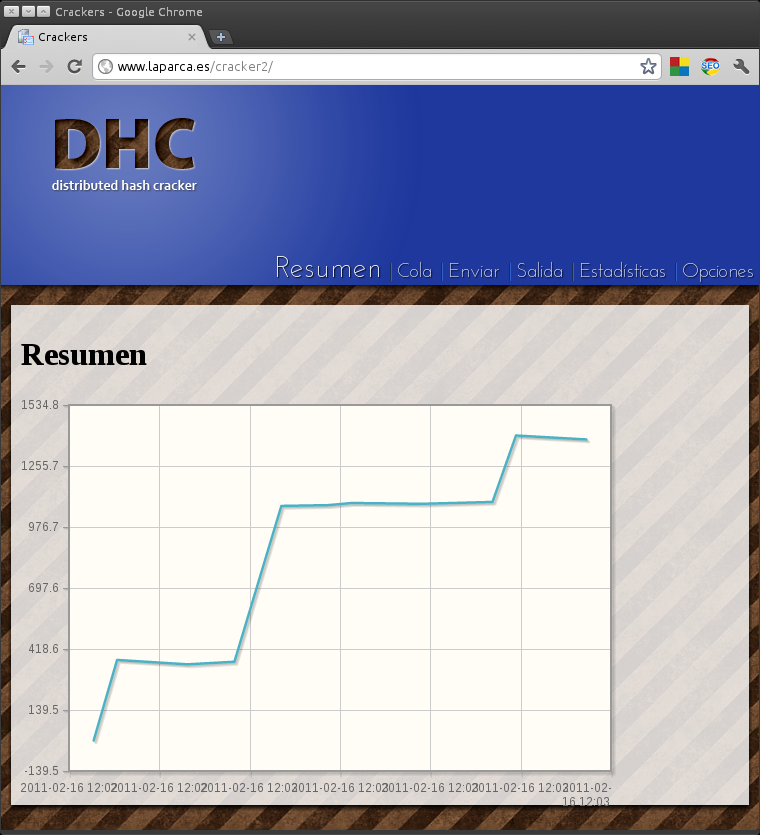
\includegraphics[width=0.7\textwidth]{images/resumen.png}
	\caption{Pantalla principal de DHC}\label{fig:DHC_principal}
\end{figure}

El primer paso es ir a enviar para solicitar la realialización de alguna tarea (ver figura~\ref{fig:DHC_enviar}). En este punto tendremos que seleccionar todas las opciones de configuración de la tarea.

\begin{figure}
	\centering
	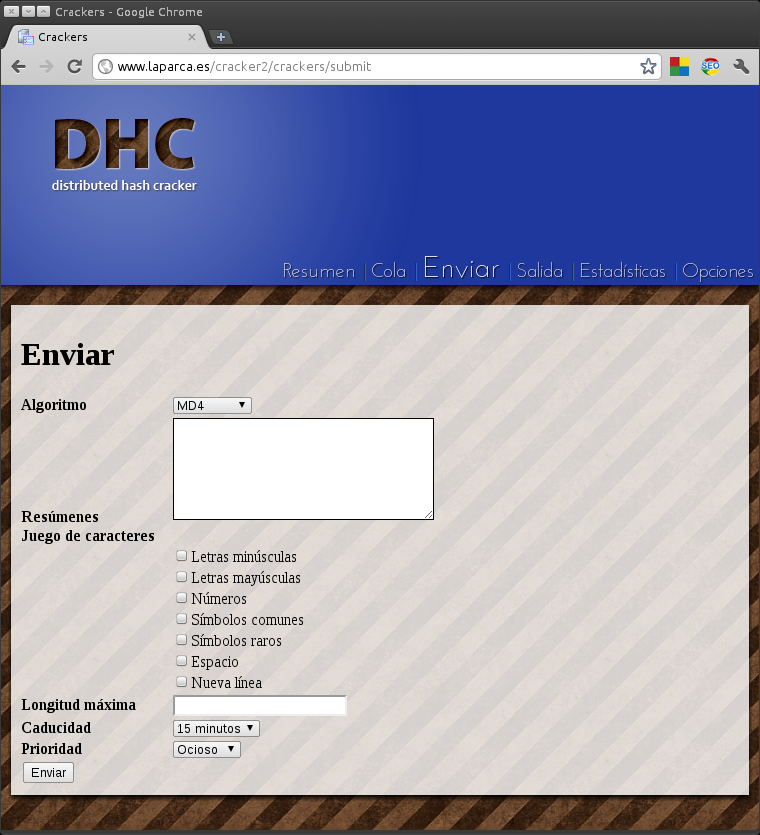
\includegraphics[width=0.7\textwidth]{images/dhc_enviar.png}
	\caption{Envío de una tarea}\label{fig:DHC_enviar}
\end{figure}

Tras el envío de la tarea el sistema nos dirá si ésta se ha almacenado correctamente o si a habido algún error.

En todo momento podemos comprobar qué tareas hay en funcionamiento desde la pantalla de cola (figura~\ref{fig:DHC_cola}).

\begin{figure}
	\centering
	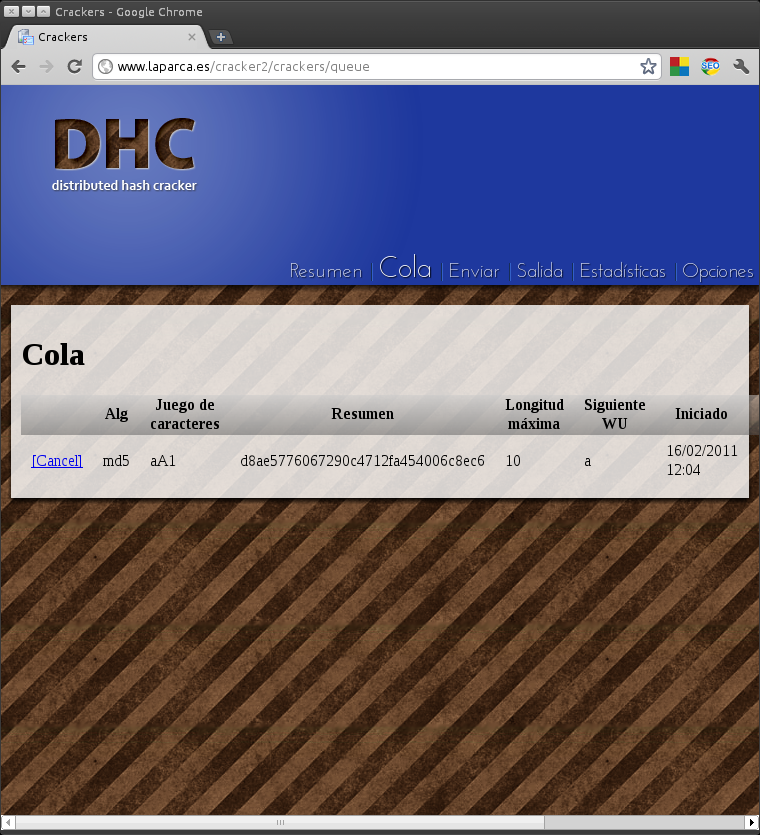
\includegraphics[width=0.7\textwidth]{images/cola.png}
	\caption{Cola de tareas}\label{fig:DHC_cola}
\end{figure}

Finalmente, podemos comprobar las tereas que se han terminado en la sección salida (ver figura~\ref{fig:DHC_salida}). Además, se puede comprobar la razón de la finalización de la tarea (resultado encontrado, no encontrado, etc.).

\begin{figure}
	\centering
	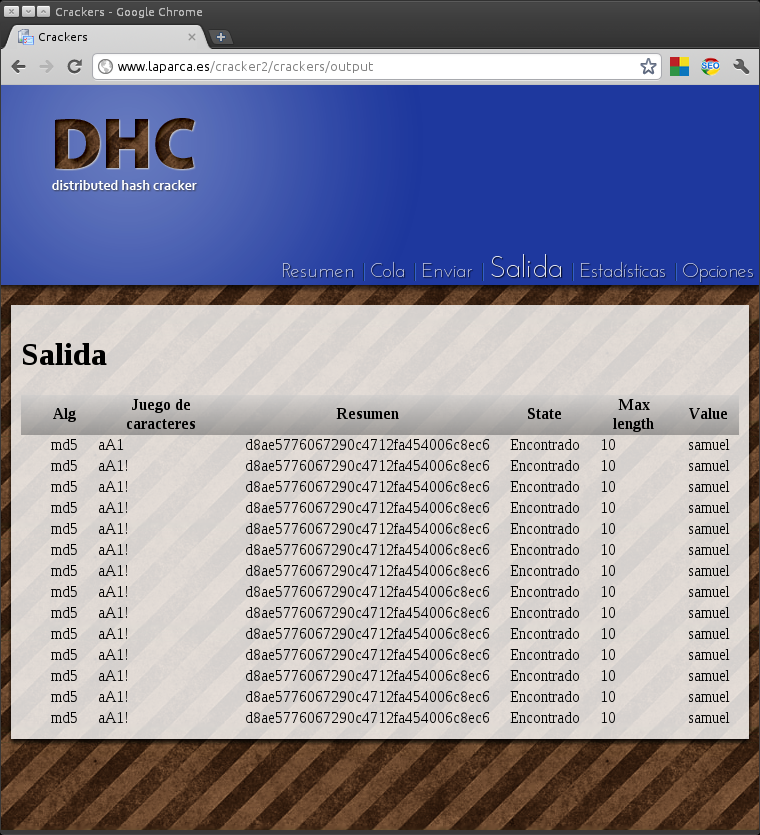
\includegraphics[width=0.7\textwidth]{images/salida.png}
	\caption{Salida de las tareas}\label{fig:DHC_salida}
\end{figure}

Si en algún momento queremos conocer mejor la situación de los agentes, se puede comprobar en estadísticas (ver figura~\ref{fig:DHC_estadisticas}) el rendimiento de cada uno y el último momento en que se ha sabido de ellos.

\begin{figure}
	\centering
	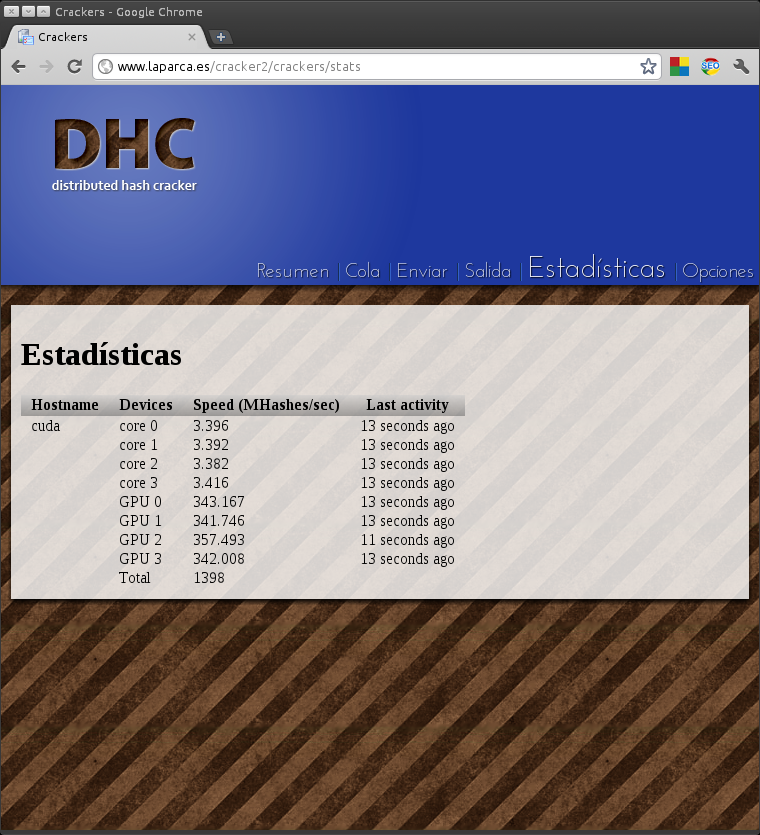
\includegraphics[width=0.7\textwidth]{images/estadisticas.png}
	\caption{Estadísticas de funcionamiento}\label{fig:DHC_estadisticas}
\end{figure}

\section{Administración de \emph{plugins}}

Durante el tiempo que esté en uso DHC pueden surgir ocasiones en las que se necesite instalar nuevos \emph{plugins} o eliminar los antiguos.  Para ello se seguirán los siguientes pasos en el agente sin olvidar que tras la modificación hay que reiniciar el agente.

\subsection{Instalación de nuevos plugins}

Para instalar nuevos plugins en el sistema solo hay que copiar estos al directorio /usr/lib/cracker/ptx. Los \emph{plugins} tienen todos la extensión .aplug.so.

\subsection{Eliminación plugins obsoletos o erróneos}

Para eliminar un \emph{plugin} con errores u obsoleto basta con borrar el fichero que lo contiene:

\begin{verbatim}
$ sudo rm /usr/local/cracker/ptr/nombre_plugin.aplug.so	
\end{verbatim}

\section{Configuraciones avanzadas}\label{sec:conf_avanzada}

En ciertas ocasiones puede hacer falta realizar instalaciones especiales de DHC. En esta sección se van a explicar dos opciones que hemos detectado.

\subsection{Varios controladores con un MySQL}
Puede darse el caso de que se necesite disponer de varios controladores de DHC pero que compartan una única base de datos. Esto puede resultar útil si la carga sobre un único controlador es muy elevada.

Para llevar a cabo este proceso se deben instalar dos o más controladores, solo con servidor web siguiendo los pasos descritos anteriormente, y a parte se configurará otro servidor con MySQL. Ambos controladores se configurarán para utilizar dicho servidor de MySQL.

Una vez que se inicien los agentes se irá pasando a cada uno la URL del controlador que deseemos o podemos configurar un balanceador de carga automático.


\subsection{Cambio de los tiempos de espera para evitar exceso de reciclado de WU}
En ciertas ocasiones, los agentes pueden tardar mucho en devolver el resultado de una WU por lo que se hace necesario modificar los tiempo de caducidad para evitar un exceso de reciclados que ralentizarían sobremedida el proceso de comprobación.

\subsection{Cambio de los directorios de búsqueda predeterminados}
Cuando un agente se inicia siempre comprueba la existencia de \emph{plugins} en unos directorios predefinidos. Además, también busca en estos mismos directorio los ficheros binarios de CUDA que le puedan ser solicitados por los algoritmos. Por defecto estos directorios son: el directorio desde el que se ejecuta el agente, el directorio \emph{ptx} desde el que se ejecuta el agente y el directorio \emph{/usr/lib/cracker/ptx}.

En caso de que se quisiese cambiar este comportamiento se puede editar el fichero config.cpp del agente para añadir o eliminar directorios de búsqueda.